\subsection{GPIO/UART/I2C/1-Wire interfaces}
\label{sec:wrpc_periph}

%\begin{figure}[ht]
%  \begin{center}
%    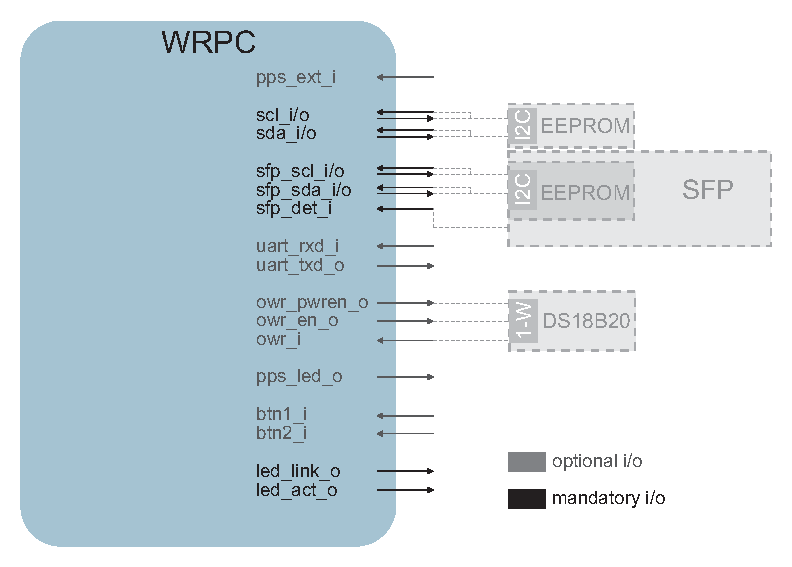
\includegraphics[width=.9\textwidth]{fig/basic_wrpc_gpio.pdf}
%    \caption{Other interfaces of WRPC}
%  \end{center}
%\end{figure}

Several hardware peripherals can be connected to the White Rabbit PTP Core. It has a UART, 1-Wire
and two $I^2C$ interfaces implemented inside. The $I^2C$ connection to the SFP module is used to
read its Part ID, while the external EEPROM stores calibration values for each supported SFP
together with an initialization script. That script is executed every time the WRPC is powered on
and can contain instructions to automatically match the SFP's Part ID with the EEPROM content and
load appropriate calibration values. The SFP presence indicator is mandatory and has to be
connected.  Otherwise, the WRPC won't be able to operate properly (without knowing whether the SFP
transceiver is actually inserted).

Furthermore, a 1-Wire digital thermometer provides on-board temperature, but also its unique ID is
used to calculate default MAC address of the physical Ethernet interface. The UART interface
provides a user shell that can be used to interact with the White Rabbit PTP Core. More detailed
description of the WRPC shell can be found in the \emph{White Rabbit PTP Core User's Manual -
  Building and Running} \cite{wrpc_man}.
